\documentclass{cumcmthesis}
\usepackage{makecell}
\usepackage{multirow}


\title{基于规划模型的农作物种植策略优化}
\tihao{C}
\baominghao{C202409001213}
\schoolname{复旦大学}
\membera{王思宇1111}
\memberb{吕天一}
\memberc{周思远}
\supervisor{}
\yearinput{2024}
\monthinput{9}
\dayinput{7}

\begin{document}

\maketitle

\begin{abstract}
农业作为乡村经济的核心产业,其种植策略的优化不仅影响着农民的收益,也对生态环境和资源的合理利用起着关键作用。本文通过建立受多种因素影响的种植策略规划模型,研究在有限的耕地资源上制定合理的农作物种植策略具有重大的现实意义。

本研究针对华北山区某乡村的农作物种植策略优化问题,旨在制定2024-2030年期间的最优种植方案,以最大化经济效益,并应对市场不确定性、政策变化及环境保护需求。在农业发展面临气候变化、市场波动和资源限制的背景下,优化种植策略对于提高农业生产效率、增加农民收入以及促进乡村经济的可持续发展具有重要意义。本文通过建立一系列数学模型,系统分析了不同情境下的农作物种植策略,并为该乡村提供了科学的决策依据和实际指导。

首先,针对问题一,我们假设未来农作物的销售量、种植成本、亩产量和销售价格保持相对稳定,构建了一个线性规划模型,将种植面积和作物种类作为决策变量,目标是最大化总收益(作物销售收入减去种植成本)。模型的约束条件包括不同类型土地(如平旱地、梯田、山坡地和水浇地)和大棚的种植限制、重茬限制(防止相同作物连续种植导致的减产)、豆类作物的种植要求(三年内至少种植一次豆类作物),以及作物产量和销售量的限制。通过求解该模型,得到了在稳定市场条件下的最优种植方案。结果显示,在所有地块合理分配作物后,总收益较2023年提升了?,并且农作物的分布更为均匀,有效降低了管理成本和风险。
\keywords{农作物种植优化,线性规划,鲁棒优化,多目标优化,不确定性分析,政策与环境因素}

\end{abstract}

\section{问题的提出与重述}
\subsection{问题的提出}
随着全球对可持续发展的日益重视,有机农业和高效农业管理逐渐成为研究的热点。现有研究表明,合理的农作物种植方案能够提高产量、降低风险,并有助于乡村经济的可持续发展\cite{ref1}。此外,农作物的生长周期、气候条件、市场需求等因素在农业管理中也越来越受到重视。优化农作物种植方案,不仅要考虑单一作物的收益,还要兼顾多种作物的合理搭配、市场需求和土地利用效率。
本文以华北山区某乡村为背景,乡村常年温度偏低,耕地类型多样。如何在有限的耕地资源上制定合理的农作物种植策略,以最大化经济效益并减少种植风险,成为亟待解决的问题。因此,本研究聚焦于华北山区某乡村的农作物种植策略优化问题,旨在通过科学的模型和方法提升乡村的经济效益。研究的核心问题是如何在未来七年(2024-2030年)内,在多种市场和环境条件下,优化农作物的种植方案,以实现经济收益最大化。
\subsection{问题的重述}
某华北乡村共有34块露天耕地,分为平旱地、梯田、山坡地和水浇地4种类型,不同地块适宜种植不同作物。此外,该乡村还有16个普通大棚和4个智慧大棚,适合种植不同类型的蔬菜和食用菌。乡村耕地的合理利用是提高收益、减少浪费的关键。此外,农作物不能连续重茬种植,每块地必须每三年种植一次豆类作物以改良土壤条件。
问题涉及农作物销售量、成本、产量等因素,要求制定2024-2030年的农作物种植方案。方案需要在多样化耕地类型和销售条件下,找到收益最大化、风险最小的种植策略。

\textbf{问题1:}要求制定2024-2030年间的种植方案,假定各类作物的销售量、成本和销售价格与2023年保持一致。在此基础上,分别针对两种情况设计最优方案:第一种情况是当某种作物的产量超过预期销售量时,超过部分将被浪费;第二种情况是当超过部分以2023年价格的50\%进行降价销售。因此需要根据不同作物的特性和地块的适宜性,平衡每季的产量与销售量,避免浪费或损失。

\textbf{问题2:}小麦和玉米的预期销售量将以5\%-10\%的速度逐年增长,其他作物的销售量变化范围在±5\%。此外,作物的亩产量将因气候波动出现±10\%的浮动,种植成本每年预计增长5\%,部分蔬菜价格也有一定上升趋势。在这些不确定性因素下,需对未来7年的种植方案进行优化,找到在收益和风险之间的平衡点。

\textbf{问题3:}进一步提出,在现实中,农作物之间可能存在替代性和互补性,销售量、种植成本和价格之间也存在一定的相关性。基于问题2的模型,需要综合考虑这些复杂的关联性,找到一套更加合理的种植方案,并与问题2的结果进行对比分析。通过模拟数据,我们可以进一步探索农作物之间的动态关系,优化整个乡村的种植策略。

具体来说,本研究将问题划分为以下几个部分:

\textbf{最优种植方案的制定:} 在假设未来销售量、种植成本、亩产量和销售价格稳定的条件下,确定各类土地和大棚上最优的作物种植组合,目标是最大化总收益。

\textbf{应对不确定性条件的优化:} 在考虑未来销售量、价格、气候变化和种植成本等不确定因素的影响下,优化种植策略以确保收益的稳定性和风险的最小化。

\textbf{综合考虑作物间关系的优化:} 进一步分析作物之间的替代性和互补性,以及销售量、价格和成本之间的相关性,制定一个综合效益更高的种植方案。

(\textbf{政策与环境因素的整合:} 纳入政策变化和环境保护要求(如碳排放和水资源限制),制定一个在经济效益、政策合规性和环境友好性方面表现最佳的种植策略。)

本研究将通过建立线性规划模型和多目标优化模型,对上述问题进行系统分析和优化。


\section{问题分析}
问题一的分析在假设未来几年农作物的销售量、种植成本、亩产量和销售价格保持相对稳定的前提下,问题的目标是为该乡村在2024-2030年期间制定一个最优的农作物种植方案,以最大化其经济效益。
\subsection{问题一的分析}
在假设未来几年农作物的销售量、种植成本、亩产量和销售价格保持相对稳定的前提下,问题一的目标是为该乡村在2024-2030年期间制定最大化其经济效益的农作物种植方案。因此,该方案需要综合考虑多种因素,包括不同土地类型的种植条件、作物的分布均匀性以及种植过程中所涉及的各种限制条件。

为实现本目标,我们采用线性规划模型,将作物种类对应的种植面积以及是否种植该作物作为决策变量,并将模型的目标函数设定为总收益,即所有作物的销售收入减去相应的种植成本,目标函数可以表示为:
\begin{equation}
    \zeta = \sum_{c=1}^{n} \sum_{r=1}^{m} (P_{c,s} \cdot Y_{c,r} \cdot A_{c,r,y,s} - C_{c,r} \cdot A_{c,r,y,s})
\end{equation}
该模型的约束条件包括多方面的要求:首先,不同类型的土地(如平旱地、梯田、山坡地和水浇地)和大棚具有各自适宜种植的作物类型,因此需限制作物的种植地;其次,需遵循重茬限制,确保同一地块内不允许连续种植相同的作物,以避免减产风险;此外,还要满足豆类作物的种植要求,即在2024-2030年期间,每个地块或大棚三年内至少种植一次豆类作物;其次,考虑到市场销售情况,每种作物的总产量不能超过其预期销售量,以避免因产量过剩而导致的滞销或降价处理的经济损失;同时,方案还需考虑作物分布的均匀性,确保种植过程便于管理,避免过于分散或种植面积过小的情况。

在模型构建中,需要假设未来几年内各类作物的销售量和价格保持稳定,每种作物的亩产量和种植成本不变。这意味着可以使用2023年的数据作为模型输入,包括各类作物的亩产量、种植成本、销售价格和销售量,以及各个地块和大棚的类型、面积和种植历史数据,这些数据将用来设定模型的参数和约束条件。

总而言之,我们需要构建一个以最大化总收益为目标的目标函数,同时建立相应的涵盖种植类型、重茬限制、豆类种植要求等多个方面的约束条件。通过使用线性规划求解算法来求解该模型,并验证结果是否符合所有的约束条件。最终,通过调整模型参数和约束条件,可以进一步优化方案,以确保其在实际操作中具备可行性和最大化经济效益的潜力。通过这样的分析方式,可以得出符合2024-2030年经济效益最大化目标的最优种植方案。



\section{模型假设}
\subsection{问题一的假设}
由于在题目给出的条件中不含有预期销售量的相关数据,我们将2023年各类作物在两季的总产量假设为2024年两季的预期销售量。对于题干中提及的“不能连续重茬种植,否则会减产”,我们认定同一年的第一季和第二季是连续的,上一年的第二季和下一年的第一季也是连续的。对于“每种作物每季的种植地不能太分散”的要求,我们假设每种作物每个季节种植的地块数不得多于5块。对于“每种作物在单个地块(含大棚)种植的面积不宜太小”的要求,我们假设每种作物的种植面积不得小于所在地块面积的30\%。
\subsection{问题二的假设}
对于题干中声称“基本稳定”的量,我们在模型中作不变处理;对于题干中声称平均年变化率为定值的量,我们将每年的变化率都取该定值;对于题干中声称平均年变化率在一个区间内波动的量,例如“平均年增长率介于5\% \textasciitilde 10\%之间”,我们假设年增长率的概率分布在该区间内是均匀的。
\subsection{问题三的假设}
\subsection{全局假设}
\begin{enumerate}
    \item 假设每年可供种植的土地面积固定且不变,不会因气候或其他因素减少。
    \item 假设在同一地块上种植的同种作物的亩产量是恒定的,不受种植面积影响。
    \item 假设每种作物的生长期不变,在同一时间段内种植的作物生长周期不受年份变化影响
    \item 假设在整个种植期内,不会发生影响农作物生长的病虫害或自然灾害。
\end{enumerate}


\section{符号说明}
以下是模型中使用的主要符号:
\begin{table}[!htbp]
    \begin{tabular}{ccc}
        \toprule[1.5pt]
        符号 & 说明 & 单位\\
        \midrule[1pt]
        $P_{c,s}$ & 指定作物在指定季节的\textbf{单位重量销售价格} & 元/斤 \\
        $Y_{c,r}$ & 指定作物在指定地块的\textbf{单位面积产量} & 斤/亩\\
        $C_{c,r}$ & 指定作物在指定地块的\textbf{单位面积成本} & 元/亩\\
        $A_{c,r,y,s}$ & 指定作物在指定地块在指定年份在指定季节的\textbf{种植面积}(决策变量) & 亩\\
        $E_{c,s}$ & 指定作物在指定季节的\textbf{预期销售量} & 斤\\
        $r$ & reduction rate & \\
        
        $\zeta$ & 总收益 & 元\\
        \bottomrule[1.5pt]
    \end{tabular}
\end{table}

\section{数据侧写}
题目提供了附件1和附件2等数据文件,虽然数据量不大,但其中涉及的各类关系相对复杂。因此,有必要对这些数据进行一个简要的分析和整理,以理清各变量之间的关联性,从而使模型构建的逻辑更加清晰和合理。此外,通过对数据的初步梳理,可以识别出关键的影响因素,确保后续的分析能够准确捕捉到作物之间的相互关系及其对收益的潜在影响,从而为制定最优种植策略打下扎实的基础。
\subsection{地块与面积分布}
不同地块的面积分布可提供对各地块可用种植面积的直观了解,有助于确定后续种植策略中的面积分配,具体如下图所示:
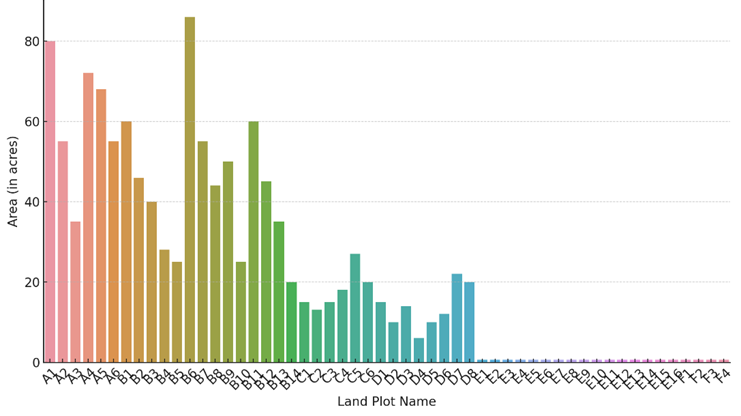
\includegraphics[width=0.5\textwidth]{image.png}


\subsection{各类型作物平均亩产量分析}

\section{准备工作/预处理}
\subsection{.csv文件的生成}
我们发现即使panda库中有read\_excel()函数可以直接读取附件中的.xlsx文件,但是其有一系列问题,例如.xlsx中合并的单元格会导致数据读取错误,只有第一个单元格的数据能被读取,并且读取的速度较慢等,因此我们选择将数据转换为.csv格式。.csv作为文本格式,相较于.xlsx格式更加方便处理。因此,我们将原始数据转换为.csv格式,以便于后续的数据处理和模型构建。src/utils/xlsx to csv/main.py中详细记录了生成.csv文件的源代码。

\subsection{full\_table.csv的生成}
在仔细阅读附件中的数据后,我们发现附件中的数据分为两部分,一部分是各类农作物的种植成本、亩产量、销售价格和预期销售量等数据,另一部分是各地块和大棚的类型、面积和种植历史数据。有一个很大的问题是为了方便后续的数据处理和模型构建,我们将这两部分数据合并为一个完整的数据表,即full\_table.csv。full\_table.csv中包含以下数据:种植地块,作物编号,作物名称,作物类型,种植面积/亩,种植季次,地块类型,亩产量/斤,种植成本/(元/亩),销售单价/(元/斤),预期销售量/斤,平均价格/(元/斤)。src/utils/generate\_full\_table/generate\_full\_table.py中详细记录了生成full\_table.csv的源代码。

\subsection{附件1\_乡村种植的农作物.csv 的格式优化}
在阅读附件1\_乡村种植的农作物.csv后,我们发现该文件中的数据格式不够规范,例如有些数据中包含了多余的空格,有些数据中的数字格式不统一等。为了方便后续的数据处理和模型构建,我们对附件1\_乡村种植的农作物.csv进行了格式优化。具体优化后的格式统一为:(([地块类型](:“第一季” (“第二季”)?)?);)+(([地块类型](:“第一季” (“第二季”)?)?))
src/utils/attachment1\_format\_optimization/main.py中详细记录了优化附件1\_乡村种植的农作物.csv的源代码。


\section{模型的建立与求解}
\subsection{问题一模型的建立与求解}
问题一要求在假设未来各类农作物的预期销售量、种植成本、亩产量和销售价格相较于2023年保持稳定的前提下,针对产量超过需求导致滞销或产量超过需求后按50\%价格进行促销的两种情况来为该乡村提供2024至2030年农作物的最优种植方案。本文首先计算预期销售量,由2023年各作物种植面积乘对应亩产量计算得到各作物的预期销售量。
在制定最优方案时,需要同时考虑如何在最小化滞销成本的同时,实现年收益最大化。此外,还需兼顾供需关系、地块面积等多种约束条件。由此可见,问题情景具有明确目标和约束条件,故可以通过建立规划模型进行求解。



\subsubsection{模型的建立}
在模型建立之前,需要定义决策变量、目标函数和约束条件,关于决策变量和相应的参数,具体如下表所示:
\begin{table}[htbp]
    \centering
    \begin{tabular}{|l|l|l|}
        \hline
        类型 & 参数 & 具体含义 \\ \hline
        \multirow{2}{*}{决策变量} & $x_{c,r,y,s}$ & 表示作物c(crop)在地块r(region)于第y(year)年第s(season)季的种植面积 \\ \cline{2-3}
        ~ & $y_{c,r,y,s}$ & \makecell{表示地块r于第y年第s季是否种植作物c的二值变量,\\加入它可以让建模过程更清晰健壮} \\ \hline
        \multirow{6}{*}{\centering 参数} & $P_{c,s}$ & 表示作物c于第s季的销售价格 \\ \cline{2-3}
        ~ & $Y_{c,r}$ & 表示作物c于地块r的单位面积产量(亩产量) \\ \cline{2-3}
        ~ & $E_{c}$ & 表示作物c的预期销售量 \\ \cline{2-3}
        ~ & $A_c$ & 表示地块c的总可用种植面积 \\ \cline{2-3}
        ~ & $M_c$ & 表示地块c的作物种植面积下限 \\ \cline{2-3}
        ~ & $C_{c,r}$ & 表示作物c在地块r的单位面积种植成本 \\ \hline
    \end{tabular}
\end{table}

目标函数为使得如下的变量最大,也即使总利润最大的函数:\\
\begin{equation}
    Total\_profit = \sum_{c, y} profit(r, s) = \begin{cases} 
        max(\sum_{c, y}(\sum_{r, s} x_{c, r, y, s} \cdot(Y_{c, r} \cdot P_{c, s} - C_{c, r})), 0), \\
            & if production(c) \leq S_c \\
        max(\sum_{c, y}(\sum_{r, s}(Y_{c, r} \cdot x_{c, r, y, s} - E_{c, s}) \cdot P_{c, s} \\
                    + \sum_{s}(E_{c, s} \cdot P_{c, s}) \\
                    - \sum_{r, s}(x_{c, r, y, s} \cdot C_{c, r})), 0), \\
            & if production(c) > S_c
    \end{cases}
\end{equation}

其中:
\begin{equation}
    production(c) = \sum_{r, s} x_{c,r,y,s} \cdot Y_{c,r}
\end{equation}

在综合研判所有提供的资料后,我们共找到了以下十三个约束条件:
1. 平旱地、梯田和山坡地每年适宜单季种植粮食类作物(水稻除外)。
2. 水浇地每年可以单季种植水稻或两季种植蔬菜作物。
3. 若在某块水浇地种植两季蔬菜,第一季可种植多种蔬菜(大白菜、白萝卜和红萝卜除外);第二季只能种植大白菜、白萝卜和红萝卜中的一种(便于管理)。
4. 根据季节性要求,大白菜、白萝卜和红萝卜只能在水浇地的第二季种植。
5. 普通大棚每年种植两季作物,第一季可种植多种蔬菜(大白菜、白萝卜和红萝卜除外),第二季只能种植食用菌。
6. 因食用菌类适应在较低且适宜的温度和湿度环境中生长,所以只能在秋冬季的普通大棚里种植。
7. 智慧大棚每年都可种植两季蔬菜(大白菜、白萝卜和红萝卜除外)。
8. 从 2023 年开始要求每个地块(含大棚)的所有土地三年内至少种植一次豆类作物。
9. 每种作物每季的种植地不能太分散。
10. 每种作物在单个地块(含大棚)种植的面积不宜太小。
11. 一种地块上种植的总面积不能超出地块面积
12. 每种作物须满足相应的种植条件,如附件1\_乡村种植的农作物.csv中所示。
13. 每种作物在同一地块(含大棚)都不能连续重茬种植,否则会减产

特别地,我们不认为每种作物的总产量不能超过预期销售量是一个约束条件,因为即使有作物的产量超过预期销售量,也有可能有其他作物因此而受益使得总利润更高,因此我们将其作为目标函数的一部分。

经过对生成的full\_table.csv的数据的仔细检查,我们发现约束1,2,4,5,6,7实际上被约束12包含,因此在代码中不再重复实现。


\subsubsection{模型的求解}
单纯形法(Simplex Algorithm)是最常用的线性规划求解算法,基于迭代移动的方法,在可行解的顶点之间跳跃,直到找到最优解。它适用于线性规划问题,并且非常有效。

在该模型的建立中,我们使用Python的pulp库中包装的线性规划求解器来实现单纯形法。具体步骤如下:

1. 定义程序意义上的目标函数和约束条件:根据模型的目标函数和约束条件,构建线性规划问题的数学表达式。

2. 使用pulp求解。

3. 进一步分析结果,检查并验证其有效性和正确性。

通过这种方法,我们能够有效地求解问题一的线性规划模型,得到在给定条件下的最优种植方案。源代码详见src/main\_1.py。

\subsubsection{数据结论}



\subsection{问题二模型的建立与求解}


\begin{thebibliography}{99}  
\bibitem{ref1} 孙飞.农作物生产专业化对农户生计的影响研究[D].中南财经政法大学,2020.DOI:10.27660/d.cnki.gzczu.2020.002168.

\end{thebibliography}
    
\end{document}
